\section{Motivation} \label{Sec:motivation}
Unlike DOM-based testing, asserting the behaviour of a \javascript application through unit-level tests requires tester to check the correctness of several intermediate code-level variables and object's properties. For this purpose, the tester needs to analyze the relation between the \javascript code and the DOM's evolution. Moreover, in order to prevent generating fragile unit tests, the testing effort should be directed towards aspects of the system behavior that are relevant to important DOM changes. We believe DOM-based assertions can be utilized as a guideline to generate unit test assertions at \javascript code level. 

\begin{figure}[!t]
  \centering
  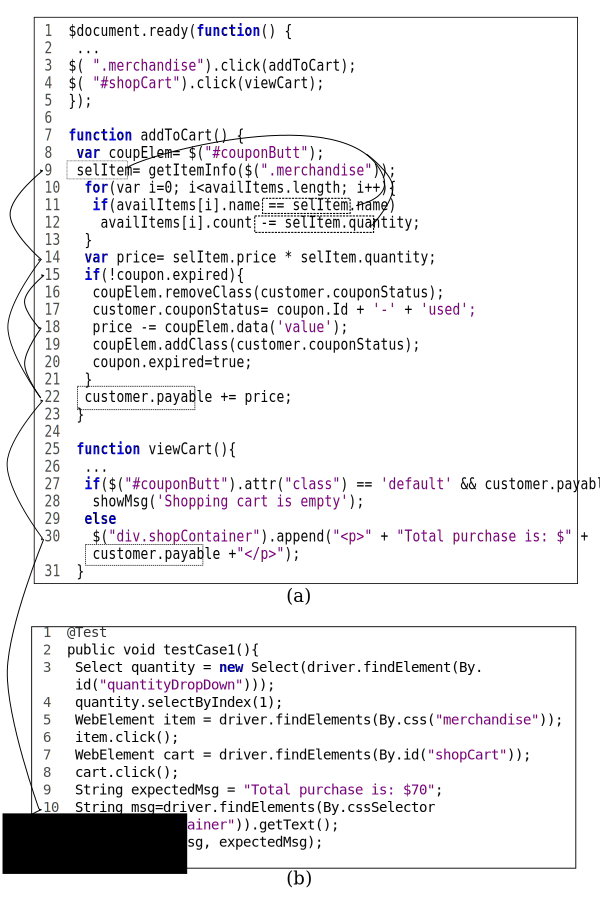
\includegraphics[width=1\hsize]{fig/example}
  \mycaption{Running example (a) \javascript code, and (b) DOM-based test case. The line from (b) to (a) shows the point of contact between the DOM assertion and the code. The arrow lines in (a) show the backward as well as forward slices between \javascript statements.}
  \vspace{-0.1in} 
  \label{Fig:example}
  \vspace{-0.1in} 
\end{figure}

\figref{example} presents a snippet of a \javascript-based shopping cart application as well as a sample DOM-based \selenium test case that we will use as a running example through out this paper. The application's code (a) contains two main functions as follows:
\begin{enumerate}
\item \code{addToCart} is bound to the event handler of DOM elements with class \code{merchandise}. When the element is clicked, \code{addToCart} gets the information of the selected merchandise, and sets the quantity of the current available items by updating the \code{availItems} object. If a valid discount coupon exists, \code{addToCart} calculates the discount value, and disables the selected  coupon button with ID \code{couponButt} by removing the corresponding class. Finally, \code{addToCart} updates the payable amount by setting the \code{payable} property of the \code{customer} object.
\item \code{viewCart} is invoked by clicking on a DOM element with ID \code{shopCart}. The function appends a message to a \code{div} element with class \code{shopContainer} including the final payable amount of the customer. If the  coupon button with ID \code{couponButt} is not selected and the payable amount is equal to zero, then the empty cart message is shown.    
\end{enumerate}
%\figref{domTest} shows a sample DOM-based \selenium test case written for the running example. 
Let's assume that in line 21 of \figref{example}(a) \code{selItem.price}, which is assigned by the original price of the merchandise is 100, and \code{selItem.quantity} is 1. In line 25, the discount, which is calculated based on the \code{data} value of the \code{couponButt} element is 30. 
The DOM-based assertion in \figref{example}(b) (line 11) checks the correctness of a text appended to a \code{div} element with class \code{shopContainer} containing the final amount payable by the customer, which is equal to 70 in this example.
Analyzing the assertion in line 11 of \figref{example}(b) indicates that the expected value of the assertion is directly influenced by the \code{payable} property of \code{customer} object as well as the object's property \code{coupon.expired} in function \code{addToCart}. We also infer that a variable in line 16 of \figref{example}(a) which directly influences the value of \code{customer.payable}, is also used in updating the value of \code{availItems.count} in line 19.

Further, by leveraging the execution information obtained from running the DOM-based test case, we can infer potentially important information about the DOM's evolution, which are not checked by the existing assertions. For instance, DOM element with ID \code{couponButt} is accessed several times in function \code{addToCart} as well as \code{viewCart} as the test case in \figref{example}(b) runs, however it remains unchecked. Since mutations of \code{couponButt} element pertains to the underlying \javascript code, it is important to assert on code statements responsible for mutating the aforementioned DOM element.             

%an expected value oracle for the given test input, confident
%that their effort is directed towards aspects of the system
%behavior that are relevant to important dom changes and thus not fragile
%
%easy to write DOM test and assert the final behaviour--difficult to write unit test and assert many intermediate behaviours that are also relevant to the final output. DOM-based tester may also miss some other important DOM-based behaviours to check.
%
%we can get more info from the sequence of events used in the dom-based test as the basis line of execution test + the dom-based assertion: from sequence we can infer missed dom checks. from dom-based assertion we can infer intermediate behaviours that are directly focused on the dom-based assertion + the rest of program points that are influenced by the assertion. this gives us an important set of oracles which falls in the neighbourhood area of the assertion, plus some important other oracles which are out of this neighbourhood zone but still important. 
 
%\begin{figure}
%\medskip
\begin{lstlisting}
	var customer = {Id:"", couponStatus:"readyToUse", shopCart:"", ...};
	var coupon = {Id:"", ...}
	...
	$document.ready(function() {
		...
		$('#couponButt').click(selectCoupon);
	});
	
	function calculatePrice(customer, coupon) {
		coupElem = $('#couponButt');
		var price= $('#merchPrice').text();
		coupon.Id = couponFromServer(url + customer.Id);
		if(customer.couponStatus != 'used'){
			coupElem.removeClass(customer.couponStatus);
			customer.couponStatus = coupon.Id + '-' + 'used';
			discountVal = calcDiscount(coupElem.data('value'), customer.Id, coupon.Id);
			price -= discountVal;	
			coupElem.addClass(customer.couponStatus);
		} 	
		customer.shopCart = price;
		$('#calcPrice').text(price);  
	}
	
	function selectCoupon(){
		...
		customer.Id = customerFromServer($('#user').val());
		calculatePrice(customer, coupon);
	}

\end{lstlisting}
\vspace{-0.1in} 

\caption{\javascript code of the running example.}
\label{Fig:example}
\vspace{-0.2in} 

\end{figure} 
%\begin{figure}
%\medskip
\begin{lstlisting}
	@Test
	public void testCase1(){
		Select quantity = new Select(driver.findElement(By.id("quantityDropDown")));
		quantity.selectByIndex(1);
		WebElement item = driver.findElements(By.css("merchandise"));
		item.click();
		WebElement cart = driver.findElements(By.id("shopCart"));
		cart.click();		
		String expectedMsg = "Total purchase is: $70";	
		String msg=driver.findElements(By.cssSelector("div.shopContainer")).getText();
		assertEquals(msg, expectedMsg);
	}
\end{lstlisting}
%\vspace{-0.1in} 
\caption{DOM-based \selenium test case.}
\label{Fig:domTest}
%\vspace{-0.2in} 
\end{figure}

